\documentclass[12pt]{report}
\usepackage[utf8]{inputenc}
\usepackage[UKenglish]{babel}
\usepackage[margin=1in]{geometry}
\usepackage{amsmath}
\usepackage{booktabs}

% images/figures/diagrams
\usepackage{graphicx}
\usepackage{subcaption}

% pre-defined macros
\usepackage{mymacros}

% line spacing
\usepackage{setspace}
\onehalfspacing

% appendicies
\usepackage{appendix}

% for changing font colour
\usepackage[dvipsnames]{xcolor}

\definecolor{darkRed}{RGB}{189, 20, 17} 
\definecolor{darkBlue}{RGB}{3, 45, 171}
\newcommand{\tcr}[1]{\textcolor{darkRed}{#1}}
\newcommand{\tcb}[1]{\textcolor{darkBlue}{#1}}


\title{An Automated Quality Control System for a Novel Production Line}
\author{jh2044}
\date{February 2020}

\begin{document}

\maketitle

\begin{abstract}
Geosynthetic Cementitious Composite Mat[ting] (GCCM) is one of a relatively new group of construction materials which enable rapid stability of ground conditions and repair of concrete structures. Concrete Canvas is a major producer of GCCM proposed a project to develop a system to monitor and minimise a perceived problem due to blockages in the cement based filler delivery lines of a new production line. Access issues meant that direct measurement in the pipe work was impossible and an indirect system based on monitoring the product further done the production line was proposed. A prototype laser profile system was constructed and tested on a small prototype line. Analysis of the initial data indicated that identification of changes to the product due to blockages was possible but the robustness was impacted by other variation in the line conditions. To understand these issues the project was modified to encompass additional tasks  1) An analysis of the whole production line  to identify potential points of failures and influences of changing the operating conditions with different product types. 2) A set of detail bench top experiments to improve understanding of the use of laser profiling of the unwoven fabric used in GCCM 3) Development of a prototype database and statistical based quality control system to take input material, line and post production measurements and provide feedback of variations and possible on Unfortunately access to the developed experimental rigs during the later stages of the project restricted collection of data. However, a prototype real-time profile measurement software has been developed and trialled on the data collected earlier. In addition, the structure of a expandable QC system has been implemented and it is hoped to have both installed before full production starts on the new line.
    
    
\end{abstract}

\tableofcontents

\chapter{Background and aim}
    Concrete Canvas is a cement impregnated composite geotextile manufacturer. They currently have two products on the market: Concrete Canvas (CC) and CC-Hydro (CCH), both of which utilise an internal spacer fabric that provides a containment void for the cement-sand powder infill. The spacer is costly due to its complicated manufacturing process. In order to enter the low cost geotextiles market, Concrete Canvas are developing a new alternative product, CCX. CCX does not include the internal spacer in its structure and only uses standard, low-cost components. Instead of the spacer fabric, CCX uses two layers of stitch bonded non-woven fabric web to create a containment void for the cement-sand powder, which is aerated and injected into the void through an array of pressurised lances.
    
    CCX is in a late \tcr{the last?} stage of development, with the final production line currently being designed, constructed and tested. The development of the final line is split into three phases: web stitching, powder injection and plastic coating with a staggered \tcr{staggered or parallel??)} development timeline across the three phases. This parallel development approach allows previous sections of the line to be tested and improved while also allowing later sections to be implemented at the same time. Additionally, line testing data is heavily relied upon in order to direct the improvement of existing sections of the line. A wide range of operating parameters are recorded during test runs of the line as well as data from destructive testing of the produced material, \tcr{but no unified framework exists to facilitate the data analysis required to optimise these parameters to produce better quality material.} \tcb{I'm trying to say that there is not much organisation of test data all together, it's all over a bunch of excel spreadsheets at the moment}. 
    
    \section{Project Motivation}
        An unexpected issue arose during the production line development with the powder injection lances becoming blocked and thus not filling the containment void sufficiently with powder, creating critically weak material. In order to unblock the injection lances, a motor controlled impulse hammer was developed to strike the lances periodically. Concerns were raised about the potential of lance fatigue being caused by the hammer impacts, so a proposal to investigate measurement systems to detect lance blockages was made with the aim of allowing the frequency and magnitude of hammer impacts to be reduced. \tcr{A preliminary investigation was carried out on site at Concrete Canvas during the Summer before the project proper began.}\tcb{(THIS IS DEFINITELY JANK, BUT NEEDS TO BE SAID SOMEHOW)}.
        
        The preliminary investigation resulted in the creation of a number of prototype systems to measure various aspects of the production line in order to infer the lance flow states. The most promising system was a laser-line projection onto the rear surface of the material web passing over a fixed roller with a video camera to reveal the surface profile. During the investigation, other issues with the existing production line became apparent; this suggested that a further investigation of the whole production line would be needed to better understand the processes involved in producing the final material, and to consider ways of controlling and optimising the product quality. 
        
        Effective control and optimisation of the quality of a manufactured product is essential in ensuring its success: a guarantee must be provided that a product will behave according to its performance specification; and by optimising the production parameters, both the quantity of wasted material can be reduced and the product performance enhanced.


    \section{Literature Review}
        The manufacture of geotextiles is a broad field with many techniques and processes involved in the production of several families of geotextiles \cite{berube2016manufacturing} with different material characteristics suited to wide range of applications in civil engineering projects \cite{ingold2013geotextiles}. Concrete Canvas specialises in the manufacture of composite geotextiles, which involves the combination of geotextiles and other components to produce a geotextile with more desirable characteristics than the individual components alone.
        
        Research has been carried out into the development of low-cost laser profilometers, similar to the prototype developed to observe the CCX surface profile such as a soil surface laser scanner which included an effective non-linear calibration scheme and extensive system performance assessment \cite{Darboux2003}, as well as a fabric wrinkle detection system which used a laser-line profilometer and statistical signal analysis to automatically grade fabric smoothness, including variation of beam incidence angle to optimise the system accuracy-resolution trade-off and profile curve fitting to remove systematic error \cite{Xu1998}.
        
        There is extensive research in the field of automatic defect detection in fabric manufacturing processes: many of the systems employ computer vision based techniques to identify the defects \cite{kumar2008computer}, such as a novel approach that estimates the fractal dimension of surface images \cite{conci1998fractal}. Approaches have been developed that use simple bilevel thresholding of images to detect very high-contrast defects \cite{stojanovic2001real}\cite{norton1993machine}, as well as more involved signal analysis of small regions of the incoming images \cite{zhang1995fabric}\cite{huart1994integration}\cite{abou2008line}. Many systems use neural networks to characterise detected defects \cite{stojanovic2001real}\cite{wong2009stitching}\cite{karayiannis1999defect} computed separately from the less computationally expensive direct statistical approaches used for real-time defect detection.
        
        Production Line Quality control systems have been developed to enhance product quality analysis by forming structural equations to represent the manufacturing processes in order to infer unknown operating parameters, and then employing various methods to optimise the product quality such as variance tolerancing \cite{suh2007dynamic},\cite{koo2001variance} and neural-networks \cite{ohshima2000quality}.
        
    \section{Aims and Objectives}
        This project investigated the CCX production line and the material it produces in order to improve the understanding of the manufacturing steps and how each one develops the material characteristics. The investigation broke down each step in the production process and established its operating mechanism, parameters that effect its operation, and also determine existing issues that result in the production of defective material. It also explored and compared a range of measurement systems to detect such defective material.
        
        An investigation of the rear surface profile of the material after the powder injection step was carried out in order to determine its key characteristics, and their distributions within both defective and non-defective material samples. Additionally, the prototype laser-line profilometer system created during the preliminary investigation was developed further to include computationally efficient detection of the incident laser line in the video footage and identification of the key characteristics of the estimated surface profile.
        
        A probabilistic model was developed to approximate the generation of the rear surface profile of the material. This model facilitates the automated detection and characterisation of defects that exist in measured material. The system was tested using samples of material both with and without known defects.
        
        A theoretical framework to unify and structure the logging of data taken from production line operation (online parameters) and destructive testing (offline parameters) was devised. The framework associates all measured parameters to the appropriate location on the produced material web, and relates parameters using a hierarchical dependence structure. This framework provides the basis for an analysis of the measured data to maximise produced material quality by optimising the production parameters.
    
    
% The new product, CCX, is a \tcr{extruded} plastic  coated two layer stitch-bonded non-woven geotextile with a cement-sand dry powder \tcr{infill}. \tcr{The/a} critical manufacturing step is a pressurised \tcr{dry} powder injection  through \tcr{280} parallel \tcr{5mm ID} aluminium tubes. This process is highly volatile and tube blockages occur creating regions of critically under-filled material. Additional failure mechanisms within the other manufacturing steps have been identified \tcr{including stitch drops etc}.
    
\section{Geotextiles}

Geotextiles represent a range of durable fabric materials with a many applications in civil engineering, due to their broad range of material properties. 
% \tcr{Geotextile materials have a wide range of applications: ditch lining, bund lining, erosion protection, the list goes on}
% Concrete Canvas and CC-Hydro \tcb{why two, what are the differences, similarities?}

% geotextiles tree
\begin{figure}
    \centering
    \includegraphics[width=0.8\textwidth]{figures/background/geotextiles_tree.pdf}
    \caption{Types of Geotextiles}
    \label{fig:geotextiles_tree}
\end{figure}

    
    \subsection{Non-woven (NW) Geotextiles}
    PET: polyethylene terephthalate
    PP: polypropelyne 
    % image of non-woven fabric (felt)
    % & image of the 3-dimensional fibre structure of non-woven
    \begin{figure}[ht]
    \begin{subfigure}{.5\textwidth}
        \centering
        % include first image
        \includegraphics[width=\linewidth]{figures/background/nw_mat_ex.JPG}  
        \caption{A typical sample of the material}
        \label{fig:non_woven_example_roll}
    \end{subfigure}
    \begin{subfigure}{.5\textwidth}
        \centering
        % include second image
        \includegraphics[width=\linewidth]{figures/background/5x_top(HH)_uncalen_comp.jpg}  
        \caption{microscope image of 3-D fibre matrix}
        \label{fig:non_woven_top_microscope}
    \end{subfigure}
    \caption{The non-woven geotextile currently used for the top surface of CCX}
    \label{fig:non_woven_example}
    \end{figure}
    
    \pagebreak
    \section{Filled Geotextiles}
    
    
    \subsubsection{Existing Concrete Canvas Products}
    % concrete-canvas existing cross sections
    \begin{figure}[ht]
    \begin{subfigure}{.5\textwidth}
        \centering
        % include first image
        \includegraphics[width=\linewidth]{figures/background/cc-illustration-high-res-1667.png}  
        \caption{Concrete Canvas (CC)}
        \label{fig:sub-first}
    \end{subfigure}
    \begin{subfigure}{.5\textwidth}
        \centering
        % include second image
        \includegraphics[width=\linewidth]{figures/background/cch-illustration-1758.png}  
        \caption{CC-Hydro (CCH)}
        \label{fig:sub-second}
    \end{subfigure}
    \caption{Cross section of existing Concrete Canvas Products}
    \label{fig:fig}
    \end{figure}

    \subsubsection{Product Under Development - CCX}
    % ccx cross sections (unlabelled)
    \begin{figure}[ht]
    \begin{subfigure}{.5\textwidth}
        \centering
        % include first image
        \includegraphics[width=\linewidth]{figures/background/set_mat_top_close.JPG}  
        \caption{Top surface}
        \label{fig:ccx_set_top}
    \end{subfigure}
    \begin{subfigure}{.5\textwidth}
        \centering
        % include second image
        \includegraphics[width=\linewidth]{figures/background/set_mat_bottom_close.JPG}  
        \caption{Bottom surface}
        \label{fig:ccx_set_bottom}
    \end{subfigure}
    \newline
    \begin{subfigure}{\textwidth}
        \centering
        \includegraphics[width=0.7\linewidth]{figures/background/set_mat_cross_section.JPG}  
        \caption{Cross Section}
        \label{fig:ccx_set_cross}
    \end{subfigure}
    \caption{A sample of hydrated and set CCX}
    \label{fig:ccx_set_sample}
    \end{figure}
    
    here is where we will briefly explain how CCX is different/better than cc normal, and offers many benefits with few drawbacks. cost saving, similar/better performance, higher production volume...
    \pagebreak
    \section{CCX Production}
            
        \begin{figure}
            \centering
            \includegraphics[width=\textwidth]{figures/background/process_flow_overview.pdf}
            \caption{Key Processes in the CCX Production Line (best viewed in colour)}
            \label{fig:process_flow_overview}
        \end{figure}
        
    \subsection{Input Materials}
        \subsubsection{Non-woven Web}
            The production line uses two non-woven geotextile webs to provide the containment surfaces for the cement blend. Properties of the web currently used in the production line are given in Table \ref{tab:nw_properties}. The NW web that is used for the CCX material is not fixed, and so the properties can change during development of the production line, and multiple products may be offered using different combinations of NW web to provide different material properties.
            The non-woven web is contained in \tcr{2000m rolls} and the web is \tcr{2.41m wide}. The rolls of the NW web are conveyed through the production line by a number of fixed position rollers, some of which are driven pinch rollers. The NW web is conveyed through the production line at an average line speed of \tcr{4m/min} which is about \tcr{250kg/hr} of web passing through the production line.
            The web conveyance path is shown in Figure \ref{fig:web_path_solid}.
\begin{table}[]
\begin{tabular}{@{}llllll@{}}
\toprule
\textbf{Surface} & \textbf{\begin{tabular}[c]{@{}l@{}}Material\\ Composition\end{tabular}} & \textbf{\begin{tabular}[c]{@{}l@{}}Thickness\\ (mm)\end{tabular}} & \textbf{\begin{tabular}[c]{@{}l@{}}Mass/area\\ (g/m\textsuperscript{2})\end{tabular}} & \textbf{\begin{tabular}[c]{@{}l@{}}MD Stiffness\\ (kN/m)\end{tabular}} & \textbf{\begin{tabular}[c]{@{}l@{}}CD Stiffness\\ (kN/m)\end{tabular}} \\ \midrule
Top              & PET:PP (9:1)                                                            & 1.37                                                              & 208                                                                 & 20.9                                                                   & 7.1                                                                    \\
Bottom           & PP                                                                      & 1.82                                                              & 237                                                                 & 16.4                                                                   & 7.1                                                                    \\ \bottomrule
\end{tabular}
\caption{NW web properties}
\label{tab:nw_properties}
\end{table}

\begin{figure}[ht]
    \centering
    \includegraphics[width=\textwidth]{figures/background/CX02 V03 side drawing.pdf}
    \caption{The NW web conveyance path along the CCX production line (excluding coating and rewind)}
    \label{fig:web_path_solid}
\end{figure}

\begin{figure}[ht]
    \centering
    \includegraphics[width=\textwidth]{figures/background/nw_unwind_far.JPG}
    \caption{The NW web unwind stands}
    \label{fig:nw_unwind}
\end{figure}
    

        \subsubsection{Yarn}
        The current yarn in the production line is a high tenacity, low shrinkage 48 filament PET thread. It has a linear density of \tcr{250 Denier(g/9000m)}. The ultimate tensile load is \tcr{12.8N} and a stiffness of \tcr{90.9N}.
        
        The yarn is unwound from 280 individual rolls as seen in Figure \ref{fig:yarn_unwind}. Each thread is then conveyed in parallel to the stitching machine via a yarn path which is confined by a number of fixed combs that direct the flow of the yarn, a section of the path is shown in Figure \ref{fig:yarn_path}.
        
\begin{figure}
    \centering
    \includegraphics[width=\textwidth]{figures/background/creole_far.JPG}
    \caption{The yarn unwind stand}
    \label{fig:yarn_unwind}
\end{figure}
\begin{figure}
    \centering
    \includegraphics[width=\textwidth]{figures/background/yarn_path.JPG}
    \caption{A section of the yarn path}
    \label{fig:yarn_path}
\end{figure}

        \subsubsection{Maliwatt Stitching Machine}
\begin{figure}[ht]
    \centering
    \includegraphics[width=\textwidth]{figures/background/maliwatt_far_crop.jpeg}
    \caption{Malitwatt stitching machine and pressure vessel (NOT ANNOTATED)}
    \label{fig:malitwatt_front}
\end{figure}

\begin{figure}[ht]
    \begin{subfigure}{\textwidth}
        \centering
        % include first image
        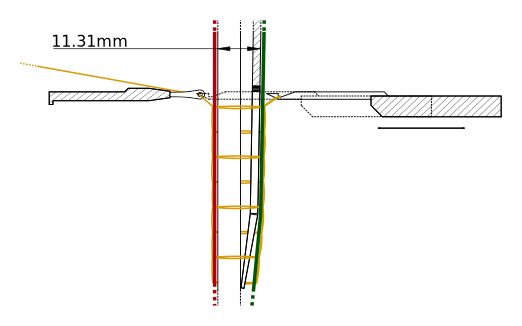
\includegraphics[width=\linewidth]{figures/background/stitch_side.pdf}  
        \caption{Concrete Canvas (CC)}
        \label{fig:sub-first}
    \end{subfigure}
    \newline
    \begin{subfigure}{\textwidth}
        \centering
        % include second image
        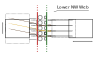
\includegraphics[width=\linewidth]{figures/background/stitch_top.pdf}  
        \caption{CC-Hydro (CCH)}
        \label{fig:sub-second}
    \end{subfigure}
    \caption{Cross section of existing Concrete Canvas Products}
    \label{fig:fig}
\end{figure}
        
\chapter{Initial Experiments}

\begin{figure}
    \centering
    \includegraphics[width=0.9\textwidth]{figures/initial_experiments/dial_far.jpg}
    \caption{Mechanical surface profile measurement setup}
    \label{fig:my_label}
\end{figure}

\begin{figure}[ht]
    \begin{subfigure}{\textwidth}
        \centering
        % include first image
        \includegraphics[width=0.8\linewidth]{figures/initial_experiments/small_mechanical.pdf}  
        \caption{small scale}
        \label{fig:dial_gauge_s}
    \end{subfigure}
    \newline
    \begin{subfigure}{\textwidth}
        \centering
        % include second image
        \includegraphics[width=0.8\linewidth]{figures/initial_experiments/med_mechanical.pdf}  
        \caption{medium scale 1}
        \label{fig:dial_gauge_m1}
    \end{subfigure}
    \newline
    \begin{subfigure}{\textwidth}
        \centering
        % include second image
        \includegraphics[width=0.8\linewidth]{figures/initial_experiments/med_mechanical_2.pdf}  
        \caption{medium scale 2}
        \label{fig:dial_gauge_m2}
    \end{subfigure}
    \caption{Dial gauge rear surface profile measurements}
    \label{fig:dial_gauge}
\end{figure}

\chapter{Production Line Investigation}

During the development of the production line, defects were found in samples of produced material. It is essential for any defects in a manufactured product to be carefully controlled for to guarantee its quality. This chapter will detail the investigation carried out to identify the types of defects that appear in the material, as well as their causal pathway. It will discuss the considerations of what measurements of the line could be made to identify these defects and the process behind the decision to use a line laser profilomter with digital camera system to detect the faults.
    
A qualitative investigation of the CCX production line was carried out in order to better understand the processes and variables involved in producing the final product. The key aim of the investigation was to identify the mechanisms responsible for producing defective material, and what additional on-line measurements could be taken in order to identify such defects automatically.
    
    \section{Injection Lance Blockage}
        \addfigure{1}{figures/line_investigation/injection_side_cutaway.pdf}{Injection Process Diagram}{injection_side}
        \addfigure{1}{figures/line_investigation/injection_front.pdf}{Injection Drawing}{injection_front}
        

\chapter{Surface Profile}


\section{Background (and possible usages linking back to sect 2\&3)}

This chapter covers the experimental investigation of the cement filled and stitched fabric that was carried out in order to quantify the effects of the identified defects on the rear surface profile of the material web after cement filling \tcb{mention the squashing of the roller here?}. The surface profile contains indications of the stitching and the cement fill as well as information about the NW web surface. This investigation continues from the initial investigation as detailed in chapter ??. 

The key aim of this investigation was to compress the large profile measurement datasets into a set of concise parameters which convey all of the relevant information about the surface profile in terms of the material quality.

\section{Bench-top Experimental Setup}

A static scanner unit was used to generate high-resolution scans of material samples which contained known defects. Samples were collected with no known defects, stitching defects, and underfill defects.

Figure \ref{fig:highres_setup} shows the scanning unit used to generate the surface profiles. Due to the scanning bed being small, the samples had to be folded to fit, as such masses were placed on the samples to ensure maximum material contact to the bed. 

The scanning unit came equipped with two stepper motor driven linear rails to facilitate precise movement of the scanning head over a sample. A software system was developed to interface with both stepper motor drivers and the laser scanner in order to automate scanning surfaces. The documented source code for automatically scanning surface areas and converting the raw data into a single Matlab or Python array file are now available alongside the scanner for future use by the structures laboratory.

\begin{figure}[h!]
    \begin{subfigure}{0.5\textwidth}
        \centering
        % include first image
        \includegraphics[width=0.8\linewidth]{figures/profile_measure/highres_setup_overview.jpg}  
        %\caption{front}
        \label{fig:highres_setup_front}
    \end{subfigure}
    \begin{subfigure}{0.5\textwidth}
        \centering
        % include second image
        \includegraphics[width=0.8\linewidth]{figures/profile_measure/highres_setup_top.jpg}  
        %\caption{top}
        \label{fig:highres_setup_top}
    \end{subfigure}
    \caption{High-resolution surface scanner setup}
    \label{fig:highres_setup}
\end{figure}

\subsection{Surface Calibration}
% bed surface calibration scan
\begin{figure}[h!]
    \begin{subfigure}{0.5\textwidth}
        \centering
        % include first image
        \includegraphics[width=\textwidth]{figures/profile_measure/typical_scatter.pdf}
    \caption{Typical surface scan}
    \label{fig:typical_scatter}
    \end{subfigure}
    \begin{subfigure}{0.5\textwidth}
        \centering
        % include second image
        \includegraphics[width=\textwidth]{figures/profile_measure/calib_surf.pdf}
    \caption{Empty bed calibration scan}
    \label{fig:empty_calib}
    \end{subfigure}
    \caption{Raw input surface scans}
    \label{fig:rot_correction}
\end{figure}




% calibration surface scan angle correction
\begin{figure}[h!]
    \begin{subfigure}{\textwidth}
        \centering
        % include first image
        \includegraphics[width=0.8\linewidth]{figures/profile_measure/uncalib_line.pdf}  
        \caption{without rotation correction}
        \label{fig:uncalib_line}
    \end{subfigure}
    \newline
    \begin{subfigure}{\textwidth}
        \centering
        % include second image
        \includegraphics[width=0.8\linewidth]{figures/profile_measure/calib_line.pdf}  
        \caption{with rotation correction}
        \label{fig:calib_line}
    \end{subfigure}
    \caption{Scanning head rotation correction}
    \label{fig:rot_correction}
\end{figure}
\pagebreak
\subsection{Data Structuring}

% \begin{figure}
%     \centering
%     \includegraphics[width=0.9\textwidth]{figures/profile_measure/typical_nw_cross.pdf}
%     \caption{Typical single scan line of raw NW surface}
%     \label{fig:raw_nw_cross}
% \end{figure}

\begin{figure}[h!]
    \begin{subfigure}{0.5\textwidth}
        \centering
        % include second image
        \includegraphics[width=\linewidth]{figures/profile_measure/typical_rear_mesh.pdf}  
        \caption{no known defects}
        \label{fig:calib_line}
    \end{subfigure}
    \begin{subfigure}{0.5\textwidth}
        \centering
        % include second image
        \includegraphics[width=\linewidth]{figures/profile_measure/fbu_01_01_top.pdf}  
        \caption{large area underfill}
        \label{fig:calib_line}
    \end{subfigure}
    \newline
    \begin{subfigure}{0.5\textwidth}
        \centering
        % include second image
        \includegraphics[width=\linewidth]{figures/profile_measure/fbu_01_02_top.pdf}  
        \caption{single tube underfill}
        \label{fig:calib_line}
    \end{subfigure}
    \begin{subfigure}{0.5\textwidth}
        \centering
        % include second image
        \includegraphics[width=\linewidth]{figures/profile_measure/fbs_06_01_top.pdf}  
        \caption{multiple stitch drop and catch}
        \label{fig:calib_line}
    \end{subfigure}
    \caption{Example defect surface scans (COULD REMOVE AXES ALLTOGETER?}
    \label{fig:rot_correction}
\end{figure}

\newpage

    
\section{Profile Parameterisation}

The raw surface provides no insight into the structure of the underlying material. In order to draw conclusions about

\begin{figure}
    \centering
    \includegraphics[width=0.6\textwidth,trim={8cm 25cm 8cm 28cm},clip]{figures/profile_measure/parameterisation_sketch.jpg}
    \caption{Current Bump parameterisation}
\end{figure}
The current parameterisation transforms any given bump to the following parameterisation (See figure above):
\begin{itemize}
    \item $\theta_1$: absolute left trough height
    \item $\theta_2$: bump width
    \item $\theta_3$: trough height difference
    \item $\theta_4$: relative height difference from trough average height to height at midpoint of bump 
\end{itemize}

\section{Raw Laser Line Image Processing}

\begin{figure}[h!]
    \centering
    \includegraphics[width=\textwidth,trim={0 5cm 0 5cm},clip]{figures/profile_measure/temp_height_measure.pdf}
    \caption{Raw Laser Line Image Processing}
\end{figure}
This process transforms each image into a calibrated estimate of the material surface. In summary:
    
\begin{itemize}
    \item Crop image to relevant region
    \item Threshold image for laser light
    \item Compute estimate for the laser height at each pixel column by comparing the light intensities
    \item Transform camera coordinates into world coordinates.
    ie $(\text{column}, \text{row}) \rightarrow (x',z')$. This requires taking into account the laser plane to camera geometry, and a simple grid calibration in the plane of the laser can be used to generate static calibration constants.
    \item transform world coordinates into material coordinates: $(x',z') \rightarrow (x,y,z)$. This requires consideration of the laser plane to material surface geometry and a correspondence between the image acquisition time and the roller movement speed/position. \tcr{Note, we will likely average over the displacement of each measurement in the longitudinal ($y$) direction for simplicity}
\end{itemize}


\begin{figure}
    \centering
    \includegraphics[width=\textwidth,trim={0 5cm 0 5cm},clip]{figures/profile_measure/temp_parameterise.pdf}
    \caption{Profile Parameterisation}
\end{figure}
This process transforms each set of surface measurement points into a set of parameters corresponding to the bumps/stitch tracks on the surface.
        
\begin{itemize}
    \item Compute stitch track locations 
    \item compute observed bump parameters $\pmb{\theta}^*_{ij}$
\end{itemize}
        
note that $\pmb{\theta}_{ij}$ corresponds to the $i$-th bump along the surface, at the $j$-th location in the longitudinal direction. also $\pmb{\theta} = [\theta_1,\theta_2,\ldots ,\theta_n]^T$ as some vector of parameters.
        
        The parameters describe elements of the bumps such as:
        \begin{itemize}
            \item width (trough-trough $x$ distance)
            \item relative height (trough-peak) height
            \item absolute height ($z$ position of troughs/peaks)
            \item curvature
            \item trough height change (trough-trough $z$ distance)
            \item surface fluffiness
        \end{itemize}
         
        This significantly reduces the size of the data-set by drawing out useful features of the profile that give an indication of the state of the observed profile in terms of its material characteristics. A careful choice of parameters is required in order to give an optimal trade-off between computational complexity and accuracy. If the parameterisation is too simplistic, it may cause not convey the required information about the surface, but too complex and the computation will be too costly to achieve a sufficiently high frame-rate.
        
        \tcr{note also that the further discretisation of the surface achieved by paramterisation does not necessarily have to be confined to bumps, but currently this seems like the most sensible unit size due to each bump containing all of the information of the material at that local region}
        



\chapter{Automatic Defect Detection}

The investigation in the previous chapters indicated that, although the measured parameters are continuous variables, there are also regions within the material that are defective. These defects are binary states, being present or not. It is crucial to identify and highlight defective sections of material as, depending on the defect, the section of material will at least need remedial work, or in the worst case, must be cut out as waste material. Additionally, certain defects must be identified in real-time, is required on the production line to resolve the defective state.

A system has been developed to identify defective sections of material based on the local parameter measurements. The identification a given defect in the material is performed through a statistical analysis of the local parameters. A parameter set has two trained parameter generation models, one representing the non-defective state, and the other representing the defective state. The likelihood of generating the observed parameters from both models are compared, and the model with the highest likelihood is the selected. Additionally, a simple defect state decision confidence is given by the difference between the likelihood of the chosen model from the other model. 

This system is superior to a direct parametric bounding to identify defective states as the failure criteria are not dependent on manually selected values, but only on the model training data, thus the more training data, the more accurate the decision boundaries will become. The only manually selected value is the decision confidence, which can be tuned to move the final decision boundary.

A pilot implementation of this system has been developed to detect and locate the presence of dropped stitches in the material web from a surface profile measurement.

\section{Concept}

For some observed parameters $\alpha = [\alpha_1, \dots, \alpha_n]^T$ we suggest that there exists a stochastic generator function $f$ from which these parameters are drawn:

\[ \alpha \sim f 
\]

See Figure \ref{fig:defect_detect_overview} for an overview of the system

\begin{figure}
    \centering
    \includegraphics[width=\textwidth]{figures/defect_detect/overview.jpg}
    \caption{Overview of the defect detection system}
    \label{fig:defect_detect_overview}
\end{figure}


\section{Stitch Drop Detection}

\begin{figure}
    \centering
    \includegraphics[width=\textwidth]{figures/defect_detect/stitch_failure.pdf}
    \caption{Stitch track failure confidence}
    \label{fig:defect_detect_overview}
\end{figure}



    \section{Profile Generation Model}
        We propose that $\pmb{\theta}$ (some bump parameterisation) is a random variable with
            \[ \pmb{\theta} \sim f(\pmb{\beta}) \]
        where $f$ is a probability density function with parameters $\pmb{\beta} = [\beta_1,\beta_2,\ldots,\beta_n]^T$ defined by the profile generating model $\mathcal{M}$.
        We assume that all bumps $\pmb{\theta}$ are independently generated. This assumption greatly simplifies the analysis. It does, however, ignore any possibility of a correlation between bump parameters in a local neighbourhood. We also assume that the parameters $\pmb{\beta}$ are also random variables with an unknown distribution. This allows the underlying generation function to change for different bumps.
        
        \subsubsection{Current Generation Model $\mathcal{M}_1$}
            The current system employs the most simple generation of the parameters which assumes that each element of $\pmb{\theta}$ is generated independently of the others with the following distribution types (the distribution type selection was based on an analysis of the nature of the parameters and also the data coming out of samples, a more convincing argument might be possible):
            \begin{itemize}
                \item $x_1$: normally distributed
                \item $x_2$: normally distributed
                \item $x_3$: normally distributed
                \item $x_4$: generalised extreme value distribution
            \end{itemize}
            each of these distributions have parameters which are contained in $\beta$.
            
            \tcr{The hope is to improve the parameterisation and to get the representation of bump height to be normally distributed as well. it is currently extreme value (long tail) because of the fluffiness generating a very large spread of possible values}
        
    \section{Model Training}
        We have a set of profile bump measurements with parameters $\{\pmb{\theta}^*_1,\ldots,\pmb{\theta}^*_N\}$ used for training model $\mathcal{M}$. In order to train the model, we perform log likelihood maximisation over the model parameters $\pmb{\beta}$:
        
        \[
            \pmb{\beta}^* = \underset{\pmb{\beta}}{\arg\max}\log\mathcal{L}_\mathcal{M}(\pmb{\beta}\mid \{\pmb{\theta}^*_1,\ldots,\pmb{\theta}^*_N\})
        \]
        
        The optimal $\pmb{\beta}^*$ then represents the best generation parameters for the training set. We manually select samples we believe were generated from different regions of the generation space (broadly nominal, stitch fail, unfilled, and different samples with new problems) and train the model for all of these sample types separately. Each of these optimised $\pmb{\beta}^*$ gives a unique generation distribution which represents the type of sample it produces. 
        \tcr{explanation of this bit is not very good, as I'm stumbling over my words}
    
    \section{Inference}
        With some set of trained bump generation parameters $\{\pmb{\beta}^*_1,\pmb{\beta}^*_2,\ldots,\pmb{\beta}^*_m\}$ representing $m$ bump generation categories, we can perform inference of the bump generating category of some test set $\{\pmb{\theta}'_1,\ldots,\pmb{\theta}'_N\}$ by comparing the likelihood that some generation parameters generated the test set:
        
        \[ 
            \mathcal{L}(\pmb{\beta}_k \mid \{\pmb{\theta}'_1,\ldots,\pmb{\theta}'_N\})
        \]
        
        we then conclude that the test set was generated with the parameters with the highest likelihood. Additionally, for the on-line system, to minimise the computational requirements, we only compute the likelihood of the nominal generation parameters given the test set. This will still give an indication of a fault in the material, but will not specify the nature of the fault.
        
    \section{Potential Issues/considerations}
        \subsection{Overfitting}
            Poor choice of $\pmb{\theta}$ may cause the model to train to a very high likelihood for the given training set, but any test set that is asserted to be a member of the same generation category will report a low likelihood of membership. 
        \subsection{Training sample data}
            Given that Concrete Canvas has a very limited knowledge of what is actually `nominal' material, it is challenging to develop a decent training set to represent this. As the currently `nominal' set contains significant parametric variance which may contain unknown faults.
            Also, given the data-set is very small, the training sets may not actually be representative of the full generation space.
        \subsection{Modelling Decisions}
            The current system proposes a `stateless' generation process, but actually there may be significant correlation between generated bumps, both spatially (across the material) and temporally (along the material). 
        \subsection{Parameter Choice}
            By discretising our surface to individual bump units, the implicit assumption is made that the bump units contain all of the relevant information for that region of the surface.
        \subsection{Noise/measurement resolution}
            All testing and development to this point has been done with the very high precision data provided by the static scanner (0.1mm $x$ and $\sim$0.5mm $y$). The minimum required resolution for the online system to draw statistically significant conclusions is unknown

\chapter{QC Analysis Parametric Framework}

This chapter reviews the work carried out to create a framework through which Concrete Canvas can carry out product quality analysis of the CCX material and production line. 

The main motivation for this work was the discovery that many useful data sources relating to the production of CCX material are currently piped into a sparse set of containers, such as notebooks or excel spreadsheets. This system is sufficient to perform basic data manipulation and analysis within a given source, but to carry out any substantial cross-source analysis is unwieldy due to the large volume of unrelated data. 

The framework proposed provides the necessary structure to pipe all data sources into a single relational database with an attached software interface, which unifies the data according to its relevant location on the produced material web rather than its time-stamp, and relates data sources according to a parametric dependence hierarchy which takes into account the order and links between production and measurement processes throughout the product's life-cycle. 

Without this framework, the best possible analysis would only be able to take into account the temporal relationship of data and any flat correlations between them. See Figure for a diagrammatic representation of this process.
\begin{figure}[ht]
\begin{subfigure}{\textwidth}
  \centering
  % include first image
  \includegraphics[width=\linewidth]{figures/qc_system/time_space_trans.jpg}  
  \caption{Time-space transformation}
  \label{fig:sub-first}
\end{subfigure}
\newline
\begin{subfigure}{\textwidth}
  \centering
  % include second image
  \includegraphics[width=\linewidth]{figures/qc_system/para_hier_dep.jpg}  
  \caption{Parametric Dependence Hierarchy}
  \label{fig:sub-second}
\end{subfigure}
\caption{Put your caption here}
\label{fig:qc_framework}
\end{figure}

\section{Time-space Transformation}

For any data source, a time series representation is trivial to produce. If a given measurement has a time-stamp, the data can be ordered accordingly. For individual sources, this is the logical frame to analyse the data, but when multiple sources from along the production process (and after production) are compared, significant temporal skew becomes an issue. For example, using a temporal frame, a profile measurement and a extruder temperature reading taken at the same moment would be directly compared, but there is potentially tens of meters of material separating them meaning significant correlation could be lost. For a more informed comparison, a real-time estimate of the effective length of final material web between various sources must be made. This will tie any reading to the cross section of produced material which it corresponds to. 

This is achievable for online readings though a conveyance model, which takes into account a utilisation factor: the quantity of each raw material (and intermediate product) that goes into the final product. The non-woven fabric will have an approximately one-to-one correspondence, whereas the yarn and cement utilisation depend directly on the stitching machine parameters which dictate the form of the final web, but simple estimates of these parameters can be drawn. 

The second consideration of the conveyance model is then to estimate the effective length of final material web between various measurement sources. Again for the non-woven, this is simply the length of fabric web between each source. The same is true for yarn except any length must be transformed by the utilisation factor. For the powder and extrudate, approximations of the volume of product within the transportation pipes must be made based on various readings. 

The more developed the conveyance model, the more accurate the location unification will be. But a very simple static model will still be a substantial improvement over a temporal model, as readings at the front and the back of the line will be separated appropriately.

A dynamic conveyance model is in development, but insufficient work has been carried out to produce a formal realisation.

\section{Parametric Dependence Hierarchy}

Assuming that the incoming data sources have the appropriate spacial unification, there is still no inter-parametric dependence. This means that any trend analysis of parameters can only consider direct correlations between them. The parametric dependence hierarchy provides a logical structure to store and interface with parameters that contains information of the dependence between them in terms of the production process.

The structure of any complex production line is a unidirectional process tree, with many source nodes representing raw input materials, and a number of intermediate nodes which represent processes that combine, modify or measure the incoming material, which lead to a final sink node representing any processes carried out on the finished product. The assumption of the parametric dependence hierarchy is that parameters of a process in the production line can depend only on parameters of earlier processes and not later processes. This significantly reduces the number of possible parameter correlations, and so provides a much more considered foundation to develop parameter inference functions. It also provides a natural investigation pathway for identified issues within materials that works backwards along the production line. For example, if a new type of defect is found by the surface profile, the state and trend of the parameters in the defective material will be considered first from the injection process, then the stitching process, and finally the raw input parameters. This simplifies the process of identifying the root cause of defects when they emerge.
\chapter{Future Work}

See figure below for the future analysis pipeline of the aforementioned QC Analysis Framework.

\begin{figure}
    \centering
    \includegraphics[width=\textwidth]{figures/future_work/qc_future.jpg}
    \caption{Future work of QC system}
    \label{fig:my_label}
\end{figure}
\chapter{Conclusions}

%Sets the bibliography style to IEEE and imports the 
%bibliography file "refernces.bib".
\bibliographystyle{IEEEtran}
\bibliography{references}

\end{document}
